
%opening
\title{Entwicklung des Layouts des Browsers}
\author{Burak Erol, Andreas Netsch, Philipp Winterholler}

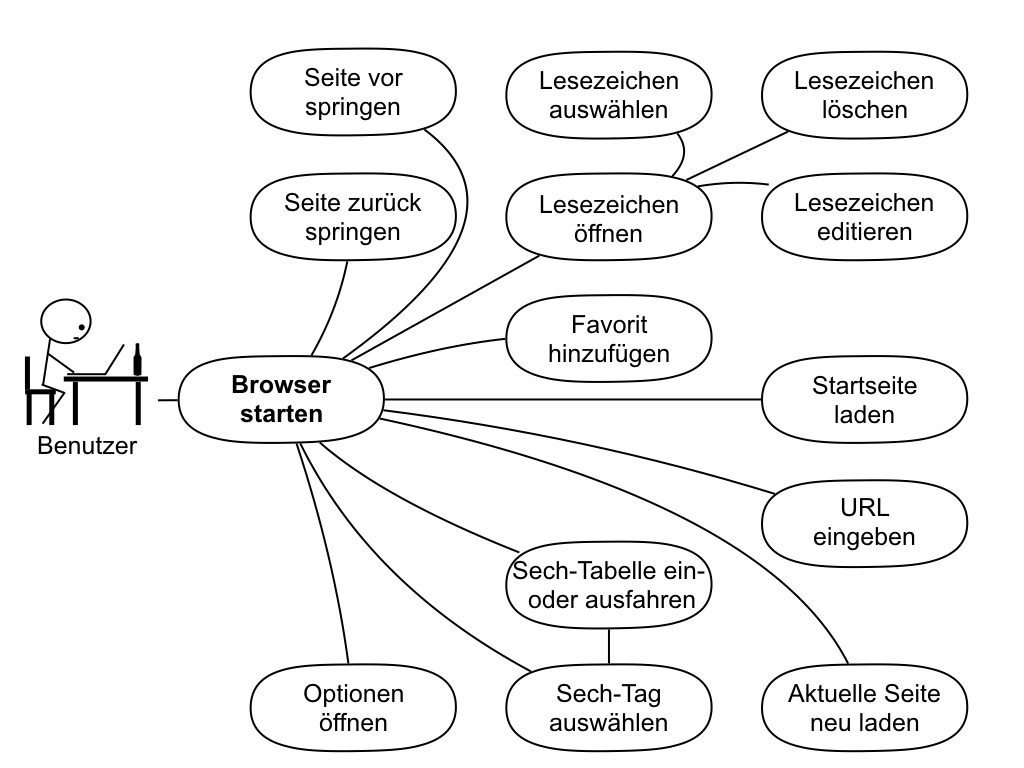
\includegraphics[width=12cm]{Pics/use_case_browser}

\section{Entwicklung des Layouts des Browsers}

Das Layout des Browsers besteht aus folgenden Elementen:

- Navigation Controller
- Navigation Bar
	- Back/Forward Button
	- Lesezeichen Button
	- Lesezeichen hinzufÃŒgen Button
	- Home Button
	- AddressBar
	- Reload Button
	- Sech Button
	- Optionen Button
- Container
- WKWebView

Die oben aufgelisteten Elemente stellen das komplette Layout des Browser dar. Der Navigation Controller dient in diesem dazu, dem Browser einen automatisch generierten Navigation Bar hinzuzufÃŒgen, welche im oberen Bildschirm fest verankert ist und eine nicht verÀnderbare Höhe und Breite liefert. Diese Navigation Bar besitzt einen Back Button, um auf einer Seite zurÃŒck zu springen und einen Forward Button, um eine Seite vor zu blÀttern. Bedient man den Lesezeichen Button so öffnet sich eine TableView mit aller gespeicherten Seiten chronologisch absteigend in der er eine Seite auswählen, löschen oder editieren kann. Will der Nutzer die Liste um ein weiteres Element ergÀnzen, so muss er den Plus Button bedienen, so öffnet sich ein Pop Up Fenster, der den Link der aktuell besuchten Seite automatisch ÃŒbernimmt und der Nutzer diesem jediglich nur noch einen Titel vergeben und abspeichern muss. Mit dem Home Button gelangt der Nutzer zu seiner definierten Startseite. Die AddressBar dient fÃŒr die Eingabe eines Weblinks der durch bestÀtigen zu der eingegeben Seite gelangt. Um die aktuelle Seite neu zu laden, muss der Reload Button bedient werden. Will der Benutzer alle Sech Tags auf der aktuellen Seite anzeigen, so bedient er den Sech Button. Ist der Sech Button angeklickt worden, so klappt sich von der rechten Bildschirmseite eine TableView mit allen Sech Tags auf und bietet dem Nutzer eine Übersicht dieser. Wird eines der Sech Tags in dieser TableView angeklickt, so öffnet sich ebenfalls ein PopUp Fenster zu diesem Tag, der weitere Informationen zurÃŒck liefert. Um die Sech Tag Tabelle wieder einzuklappen wird ein weiteres Klicken auf den Sech Button benötigt und diese fÀhrt sich ein. Durch einen Klick auf den Optionen Button öffnet sich auch hier ein Pop Up Fenster, der benutzerspezifische Informationen mitliefert und ÃŒbersichtlich darstellt. Um den WKWebView eine dynamische Höhe und Breite programmatisch zu ÃŒbergeben, wurde ein Container, eine Schicht unter diesem, mit festen Constraints ÃŒbergeben. Diese Constraints passen sich zu den benachbarten Elementen, wie der ausgefahrenen Sech Tabelle oder der Navigation Bar, an und das WKWebView ÃŒbernimmt die Constraints dieses darunter liegenden Containers. Dreht man das EndgerÀt beispielsweise von Hochformat in den Querformat, Àndern sich Höhe und Breite des Containers und diese werden vom WKWebView ÃŒbernommen.

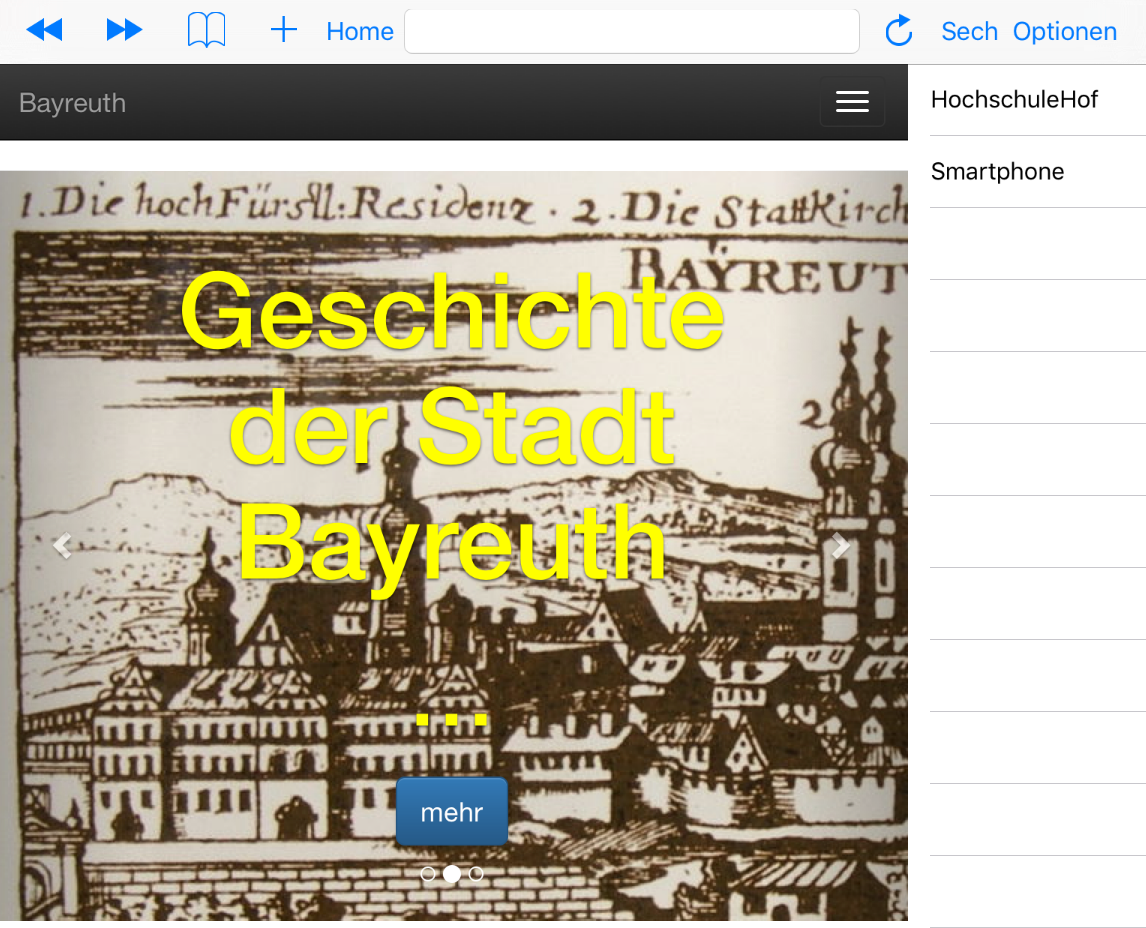
\includegraphics[width=12cm]{Pics/Browser_Hochformat}


